%%% template.tex
%%%
%%% This LaTeX source document can be used as the basis for your technical
%%% paper or abstract.

%%% The parameter to the ``documentclass'' command is very important.
%%% - use ``review'' for content submitted for review.
%%% - use ``preprint'' for accepted content you are making available.
%%% - use ``tog'' for technical papers accepted to the TOG journal and
%%%   for presentation at the SIGGRAPH or SIGGRAPH Asia conference.
%%% - use ``conference'' for final content accepted to a sponsored event
%%%   (hint: If you don't know, you should use ``conference.'')

\documentclass[review]{acmsiggraph}
\usepackage{fixltx2e}
%%% Make the ``BibTeX'' word pretty...

%%% Used by the ``review'' variation; the online ID will be printed on 
%%% every page of the content.

\TOGonlineid{45678}

%%% Used by the ``preprint'' variation.

\TOGvolume{0}
\TOGnumber{0}

\title{SVGPU: Real Time 3D Rendering to Vector Graphics Formats}

\author{Apollo I. Ellis and Warren Hunt and John C. Hart}
\pdfauthor{Stephen N. Spencer}

\keywords{3d, vector graphics,real time rendering, GPU}

\begin{document}

%%% This is the ``teaser'' command, which puts an figure, centered, below 
%%% the title and author information, and above the body of the content.

 \teaser{
%    \includegraphics[height=1.5in]{images/sampleteaser}
%   \caption{Spring Training 2009, Peoria, AZ.}
 }

\maketitle

\begin{abstract}

Rendering realistic 3D scenes to vector graphics in real time has not yet been explored in modern graphics research. Display resolutions have begun to grow rapidly and a resolution independent renderer may thus become interesting. Further in the advent of cloud gaming raster images for large displays will prove a significant bottleneck when being transported over networks from server to client.  Most prior efforts have either achieved sub real time performance or focused on single image generation. We implement a real time rendering pipeline that utilizes a novel analytic visibility algorithms to output a compact vector graphics representation of a 3D scene. Our system is fast and efficient on modern hardware and thus enables the benefits vector graphics representations to reaped by the real time community.

\end{abstract}

\begin{CRcatlist}
  \CRcat{I.3.3}{Computer Graphics}{Three-Dimensional Graphics and Realism}{Hidden line/surface removal}
  \CRcat{I.3.7}{Computer Graphics}{Three-Dimensional Graphics and Realism}{Visible line/surface algorithms};
\end{CRcatlist}

\keywordlist

%% Required for all content. 

\copyrightspace

\section{Introduction}
In the earliest days of computer graphics, the VRAM needed for a raster
framebuffer was prohibitively expensive, and graphics was output in a vector
format. Hidden line algorithms were needed to convert 3-D scene geometry into
a planar map of view projected regions with depth complexity one, so their
outlines could be displayed on the vector display devices available then. Even
though raster displays have been available for decades, the output of 3-D
scenes as a vector planar map is still a valuable process for many
applications. For example, the rendering of 3-D scenes as line art and other
non-photorealistic rendering approaches are based on the extraction of
silhouettes and visible regions as planar maps, e.g. \cite{lineart,npr}.

As the output of a 3-D scene renderer, a planar map image of 2-D polygons has
several advantages over a raster image of pixels. First, vector images provide
a resolution independent representation that can be efficiently rasterized at
any resolution onto an arbitrarily sized display, ranging from watches to
videowalls to head-mounted displays. The rasterization of a planar map consists
of point-in-polygon
tests and avoids the need to sort depth, and so does not suffer the
pathological issues of depth buffering \cite{wmap,etc}. Moreover, the planar
map vector image allows rasterization to be delayed until display, so the
display's resolution can be accomodated, and proper edge antialising can be
performed.

Second, in an era where wireless network bandwidth is a critically
valuable commodity, vector images are compact, reducing both network
consumption and latency. Cloud gaming is an emerging trend of the video gaming
industry, where the display image of a video game is rendered by a server and
transmitted over the internet to a thin client. Current gaming-as-a-service
(GaaS) systems render raster images that are transmitted as MPEG streams, but
these streams consist of full resolution I-frames because the computation of
block motion on these raw images needed for more efficient MPEG transmission
creates too much latency. A server rendering 3-D game scenes directly to a
planar map yields correspondences that would better support motion for more
efficient game video transmission.

Auzinger et al. \cite{auzinger2013} showed that the computation of analytic
visibility can be practical on the GPU with an edge-based renderer. They
showed that analytic visibility could be computed faster than the
multisampling needed to properly rasterize some pathological cases.

In this paper we present a real-time triangle-based vector renderer that
converts a 3-D meshed scene into a planar map of 2-D triangles. This result can
be directly converted into a vector graphics representation (e.g. SVG)
or can be quickly rasterized without need for a depth buffer and with
display-resolution-dependent edge antialiasing such as MLAA, SMAA and CMAA
[define these]. This system also extracts the
visual contour as well as the regions it bounds, and both can be easily
stylized for non-photorealistic rendering.

\begin{figure*}
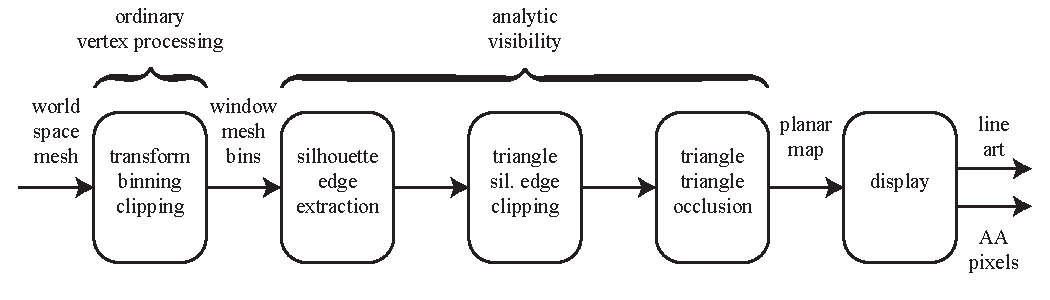
\includegraphics{images/pipeline.pdf}
\caption{The stages of our binned vector graphics rendering system.}
\label{fig:pipeline}
\end{figure*}

Our pipeline consists of 5 stages. The first stage, transform, clipping, and
binning is borrowed directly from the rasterization pipeline. Our system makes
no noteworthy additions to these stages. The next three stages make up our
analytic visibility pipeline. The first stage of analytic visibility, second
over all, is silhouette extraction via hashing. Silhouettes are computed as
triangles with neighbor-less edges or triangles with oppositely signed normal
vectors that share an edge. In the third stage the triangles in each bin are
clipped to the silhouettes in that bin.  This simplifies the next pipeline
stage significantly by eliminating the need for brute force triangle vs
triangle clipping. In the fourth stage a discard test is performed on each
triangle by clipping it against the other triangles in the bin. The clip here
is simplified to a would-clip and discard test, since all silhouette edge
clipping operations have already been resolved. In the fifth stage our system
has the choice of either converting to a vector graphics format or rendering
vertex interpolated values via rasterization.

The design of our vector renderer is based on the idea that we use the same
spatial coherence and streamed processing tricks developed for fast
rasterization graphics pipelines to accelerate the rendering of vector
graphics. These tricks include binned rendering and spatial hashing, as well
as load balancing and tuning.

% The visibility pipeline must feature every visible surface, there should be no
% overlap, and it must output geometry which can be rendered to produce a scene
% faithful to one rasterized with vertex attribute interpolation. The hidden
% surface element is solved in our system by a sequence of categorization and
% clipping operations. The clipping operations in turn satisfy the no overlapping
% condition [TODO:rephrase]. Since the visibility operations remove all hidden
% elements accurately (analytically) and leaves all visible geometry, we
% faithfully represent the scene in 2D. This planer map may be rasterized
% without condideration for depth in such a way that it is indistinguishable
% from an image produced by a traditional raster pipeline.  This analytic
% pipeline has complexity on the order of the geometry, rather than the order of
% the resolution of the final image and becomes relatively more efficient as
% final render target resolution increases.

\section{Previous Work}
TBW
\begin{itemize}
\item Rendering to Vector Graphics 
\begin{itemize}
\item Elmar Eisemann, Sylvain Paris, and Frédo Durand. 2009. A visibility algorithm for converting 3D meshes into editable 2D vector graphics. 
\item Clip art rendering of smooth isosurfaces. Matei Stroila, Elmar Eisemann, John Hart
\item EISEMANN, E., WINNEM¨O LLER, H., HART, J. C., AND SALESIN, D. 2008. Stylized vector art from 3d models with region support.
\item RYU, D. 2001. Visibility Layer Decomposition. Senior thesis, Harvard University.
\item Snaxels on a Plane Kevin Karsch John C. Hart 
\end{itemize}
\item Analytic Visibility
\begin{itemize}
\item Thomas Auzinger, Michael Wimmer, Stefan Jeschke Analytic Visibility on the GPU
\item Wavelet Rasterization. J  Manson and S. Schaefer
\end{itemize}
\item Anti aliasing
\begin{itemize}
\item Alexander Reshetov. 2009. Morphological antialiasing. In Proceedings of the Conference on High Performance Graphics 2009 (HPG '09)
\item AUZINGER T., GUTHE M., JESCHKE S.: Analytic Anti-Aliasing of Linear Functions on Polytopes.
\end{itemize}
\item Legacy 
\item Analytic
\begin{itemize}
\item Edwin Catmull, A Hidden-Surface Algorithm with Anti-Aliasing
\end{itemize}
\item Depth Buffer
\begin{itemize}
\item A Subdivision Algorithm for Computer Dis-play of Curved Surfaces
\end{itemize}
\item Hierarchical Z
\begin{itemize}
\item Hierarchical Z-Buffer Visibility Ned Greene Michael Kass Gavin Miller
\end{itemize}
\item BSP
\begin{itemize}
\item On visible surface generation by a priori tree structures H Fuchs, ZM Kedem, BF Naylor
\end{itemize}
\item Surveys
\begin{itemize}
\item A survey of practical object space visibility algorithms  S Ghali
\item A SURVEY OF OBJECT-SPACE HIDDEN SURFACE REMOVAL SUSAN E. DORWARD
\item Charles W. Grant. Visibility Algorithms in Image Synthesis
\end{itemize}
\end{itemize}

\section{The SVGPU Pipeline}

We make assumptions about the input geometric data and scene to simplify our pipeline design, but acknowledge the need to break these assumptions in the future to support arbitrary geometric data and scene topologies. Firstly it is assumed that the input is an indexed face list, this simplifies our hashing functionality for silhouette edge extraction. Secondly, it is assumed that triangles do not pierce each other, this simplifies the clipping operations. Lastly it is assumed that if a triangle has no neighbor on some edge side then that edge of the triangle can be safely categorized as a silhouette edge and there is no need to fuse any neighboring geometry nearby to that edge. This simplifies silhouettes extraction via hashing.

\subsection{Extracting Silhouettes}
Extracting silhouettes should be simple, fast, and effective. So a hash based approach is employed which is easy to implement, can be parallelized on GPUs, and provides the analytically correct silhouette edges. The hash key is based on the indices from the indexed face set in pairs of two per edge. Note that spatial hashing would also work in the case where the input is triangle soup, but an index face set in used in the experiments in this paper. The hashing stage requires hash key computation, silhouette edge detection on hash collision, and hash table writes.
\\\\
First a hash key must be computed for each edge and then hashed to detect silhouette edges. For each pair of two 32 bit indices the bits are interleaved and the result is moded by a large prime number [TODO:why do we mod by a large prime?]. If the two indices were instead appended together the hash location would largely depend only on the lower order index which may produce a bad hash function. So interleaving is used. The next step is to check if there are other edges in the hash location and if so compare the z values of the normal associated with two triangles sharing an edge. If the normal vectors are a positive-negative pair this edge is marked as a silhouette. Otherwise the edge data is written into the hash table bucket at that key’s location. 
\\\\
As previously stated computing silhouettes is important to our pipeline because it simplifies the clipping computations needed to compute analytic visibility. Silhouettes have additional benefits to rendering, as previously mentioned. Silhouette processing simplifies the computation in two ways. Now the system only needs to compute the clipping of each triangle against one edge at a time, the silhouette edges. Alternatively it would be necessary to compute a full triangle vs triangle clip or clip multiple edges against multiple edges as in previous approaches. Secondly, each triangle has already been clipped against all possible silhouette edges so there is no need to perform a full clip in the next stage. It becomes sufficient to check if a triangle begins to clip or “would clip” another triangle. If this is the case it’s ok to discard the other triangle because if one triangle partially occludes another that triangle must be a silhouette edge and those cases are handled first.
\\\\


\subsection{Triangle vs Edge Clipping}
	In this stage the goal is to clip every triangle in a bin to the all the silhouette edges in that bin. The act of actually clipping a triangle to a silhouette edge occurs much less frequently than the act of discounting the need to clip a triangle against any of the silhouette edges. Further since clipping a triangle to a silhouette edge may produce new triangles that would then also need to be clipped by edges, this stage has been segmented to retain instruction execution coherence on GPUs.
\\\\
To check for clipping three tests are employed. The first is a point on edge side test. If the test returns a non-trivial result, i.e. different vertices fall on both sides of the edge the stage proceeds, otherwise it returns. Proceeding is to compute the intersection points at which triangle crosses the silhouette edge. The z values of these points are then checked against the z values of the corresponding xy locations on the silhouette edge’s triangle plane and the algorithm returns if these intersection points are in front of the plane. Lastly it is necessary to check if the intersection points lie either inside the silhouette edge interval or on opposite sides. The second case accounts for a silhouette edge which lies completely inside a partially occluded triangle. If neither occurs the algorithm returns, but if it did not return early the triangle is marked as needing to be clipped by the second segment of this stage.
	\\\\
In the second segment a full and triangle vs edge clipping must occur, which may generate new geometry. The new geometry may require additional clipping. Essentially there may exist a triangle that is clipped by an edge and then in turn the new geometry is clipped by other silhouette edges. This requires care in parallelization to handle load balance but our algorithm is fairly straightforward [TODO: straitforward? does it achieve load balance?].
\\\\
To clip a triangle against an edge is as follows. First it must be determined which edges overlap the silhouette edge. In the case where the two edges overlapping are extending from one vertex, the algorithm clips off the un-occluded triangle region, divides the remaining region in two triangles, and writes all three back into a buffer for further clipping by other edges. In the case where the two edges are extending from two different vertices the inverse operation occurs, clipping off a two triangle quad, and writing back these and the left over triangle to a buffer for further processing. The algorithm is simple and can be implemented efficiently on a GPU. However, again, the GPU implementation will take some care in design to avoid load imbalance.


\subsection{Occlusion}

	The last phase of our visibility infrastructure consists of checking triangles for occlusion by other triangles. This check is a simplified version of triangle-triangle clipping. A similar method as in the first segment of triangle vs silhouette edge clipping is used here. The only information needed is whether a triangle would need to clip a given triangle, in fact the tests are exactly the same as before. The triangle id is written to a visible list if the algorithm did not return early (e.g. because it would have needed to clip).

\section{Implementation}
We implement our pipeline primarily on the GPU using Cuda kernels with some CPU orchestration. Vertex shading and clipping are separate kernels. One kernel computes model view projected vertices, and the next assembles triangles checks if they need be to clipped to z cross 0 plane. If clipping is needed then any newly generated clip geometry is written into a buffer for binning and divide by w also occurs in this kernel. Now the triangles must be binned by bounding box. Triangle vertex data is stored in the bins along with id, simplifying the kernels in further stages. The binned triangles contain four floats per vertex with indices packed into w, and a face normal.
\subsection{Silhouette Hashing}
The implementation here is straightforward GPU based hashing over the entire input set. Since the complexity of this operation is somewhat independent of bin size, all edges in the screen are hashed in the same kernel. An m by n kernel is launched where n is the number of bins and m is the total triangle count divided by n. Each column of threads in the grid is reading from one bin.
\\\\
Our kernel calculates hash keys by interleaving the index bits, hashes edges, and marks silhouettes. An edge is not always written into the hash table, the write requires GPU atomics to increment counters for the hash buckets associated with the keys. Better to not do an atomic if not necessary, so the write happens only after checking hash table contents for adjacent edges. If the edge’s pair is not available it will have to be written and read back by a different thread [TODO: is there a race-condition here?]. If it is available the z values are compared and if they are oppositely signed it is marked. To mark a silhouette edge the kernel writes its id into a buffer location indexed by an atomic counter. 
\\\\
This leaves the problem of marking unmatched edges as silhouettes, so during hashing a flag is set on the hash table every time a location gets an edge, de-asserting when an edge pair is found, and re-asserting when another edge arrives. After the kernel returns a cleanup kernel writes back any edges left behind. NVidia’s compute model 3.5+ dynamic parallelism is used here but the discussion is left for the next section where its usage is more critical to our implementation.


\subsection{Triangle vs Edge Clipping on the GPU}
As mentioned the triangle vs edge clipping phase is cut into two segments, a categorization segment, and a clipping segment. In the first segment an m by n kernel is launched to the GPU to clip m triangles against n edges. Each thread m\textsubscript{i}n\textsubscript{j} is responsible for determining whether a triangle  m\textsubscript{i} is clipped by edge n\textsubscript{j}. If this is the case the kernel writes out the triangle id to a list for further processing. As mentioned in the algorithm section if this is not the case the thread retires. This kernel is simple, but the kernel that follows is much more complex due to a load balancing problem.
\\\\
In the second segment triangle vs edge clipping operations occur which can generate additional operations. To balance the work on the GPU a work queue method based on dynamic parallelism is used. Dynamic parallelism, available on Nvidia’s compute model 3.5+ GPUs, affords us the ability to launch a kernel from within a kernel to avoid expensive CPU-GPU synchronization, data transfers, and driver overhead. Kernels are launched in rounds where each round determines how many threads to enque to the next round based on the work generated.
\\\\
The first kernel clips all triangles from each bin that contained silhouettes with a single silhouette edge from each bin. Recall that as a triangle is clipped against an edge it generates one or two new triangles and writes them to storage. If there are more edges in a bin a kernel always enques three threads to the next round kernel, one for each clipped triangle region. Care is taken to write the new triangles back to a location index-able in the next phase by the so called child threads of the current phase. In that next phase each child thread reads its triangle based on its newly generated thread id and the next edge to process is accessed from a list via an atomic counter. The deeper details of the id based look up scheme are beyond the scope here, but the interested reader is encouraged to refer to Nvidia’s Cuda Compute API 3.5+ for more on dynamic parallelism. 

\subsection{Occlusion Pass}
This phase operates in a single kernel and reuses code from the triangle vs edge clipping section. If it is determined that there would be need to clip a triangle is it discarded. The kernel is m by m by n grid where m is the number of triangles in a bin and n is bin count. For reference the bin size used is 128x128 pixels. While this phase is simple it is also fast, a byproduct of the main contribution of our silhouette based algorithm, simplified clipping.

\subsection{Rendering}
At this point in the pipeline there two options, render directly, or send to a client. Our rendering implementation invokes OpenGL with the depth buffer disabled and uses a pass through vertex shader. Phong shading is implemented in the pixel shader. It follows from this that the system has met the goal of representing the scene as a planar map since it OpenGL can effectively render our output directly. To further show validity as a vector graphics format a rendering backend that uses the Nvidia’s path rendering API is also in place.

\section{Results}



 
\section{Discussion}
As mentioned we envision a client server model equipped with our system. We imagine this either as a cloud server serving to a low-power machine or, similarly, a powerful machine streaming to a VR HMD. In these model a scene would be submitted to the pipeline server which proceeds to transform, clip, and perform our custom visibility outputting a planar map representation. Then the scene can be sent to the client in its compact form with low latency. The client could avoid all depth-related computation and need only be able to perform point in polygon tests, interpolation, and fragment shading. This hypothetical rasterizer doesn’t even need a z buffer. So it would be consuming almost no bandwidth. [TODO: Not sure I buy this argument.  Due to z-compression, z-buffer bandwidth isn't extreme relative to texture or g-buffer bandwidth used during shading computations]
\\\\
There are a few important limitations in our system. One, is pixel shaded images must be generated by running a pixel shader on the output of a rasterization of our output. Two, texture mapping must be handled in the same way and this would eliminate the argument that our format is compact yielding low latency transfers. However, textures could be streamed to the client once and reused for many frames.  Textures could also be compressed or regioned. There is also work on generating vector graphics representations of textures, but the texturing problem is left as future work.
\\\\
Shadows are of great interest in real time applications and it is desirable to make them work in our infrastructure. Shadow volumes are a promising approach because they can be computed analytically and stored in a vector graphic format. Soft shadow volumes could potentially be embedded as well with a blend layer, and we have work ongoing in this area. Indeed the idea of representing layered vector graphics and interpolation schemes is not in any way out of scope for the continuation of this project. [TODO: transparency?]

\section{Conclusion}
plus future work.

\section*{Acknowledgements}

No acknowledgments in review version.

\bibliographystyle{acmsiggraph}
\nocite{*}
\bibliography{template}
\end{document}
